%!TEX root =  main.tex

\lectureheader{162}{Calculus II}{Inverse trigonometric functions}{\textit{Thomas' Calculus}  7.6}

\begin{remark}
The trigonometric functions are periodic, and so they can't have inverses.
So, we do the best that we can. 
As with the square and square-root, we invert a preferred ``slice" of each.
\end{remark}

\begin{example}
For each of the six trigonometric functions, identify an interval of the domain for which the function is one-to-one and onto its full range.
\end{example}
\ifdefined\SOLUTION
\SOLUTION[Solution]{
Picture the graph of each in your mind.
\begin{enumerate}
\item The function $y=\sin x$ is increasing and one-to-one on the interval $[-\pi/2, \pi/2]$.
Furthermore, the function attains every (output) value in the range $[-1,1]$ exactly once as $x$ varies in $[-\pi/2, \pi/2]$.
\item It follows that $y=\csc x$ is one-to-one and onto its range over the union $[-\pi/2, 0)\cup (0,\pi/2]$.
\item The function $y=\cos x$ is decreasing and one-to-one on the interval $[0, \pi]$.
Furthermore, the function attains every (output) value in the range $[-1,1]$ exactly once as $x$ varies in $[0, \pi]$.
\item It follows that $y=\sec x$ is one-to-one and onto its range over the union $[0, \pi/2)\cup (\pi/2, \pi]$.
\item The function $y=\tan x$ is increasing and one-to-one on the interval $(-\pi/2, \pi/2)$.
Furthermore, the function attains every (output) value in the range $(-\infty, \infty)$ exactly once as $x$ varies in $(-\pi/2, \pi/2)$.
\item For $y=\cot x$, we may use the interval $(0,\pi)$.
\end{enumerate}
}
\else
\fi

\newpage

\begin{definition}
The six ``inverse" trigonometric functions are defined by the rules:
\begin{enumerate}
\item $y=\arcsin x \iff \sin y = x$ and $y\in [-\pi/2, \pi/2]$.
\item $y = \arccos x \iff \cos y = x$ and $y\in [0,\pi]$.
\item $y = \arctan x \iff \tan y = x$ and $y\in (-\pi/2, \pi/2)$.
\item $y=\arccsc x \iff \csc y = x$ and $y\in [-\pi/2, 0)\cup (0, \pi/2]$.
\item $y = \arcsec x \iff \sec y = x$ and $y\in [0, \pi/2)\cup (\pi/2, \pi]$.
\item $y = \arccot x \iff \cot y = x$ and $y\in (0,\pi)$.
\end{enumerate}
\end{definition}
\begin{remark}\,
\begin{itemize}
\item We call them inverse trigonometric functions, but that's really a lie!  They're impostors!
\item Even though I don't like it, we will also use the alternative notation $\sin^{-1} x = \arcsin x$, $\cos^{-1} x = \arccos x$, etc.
\end{itemize}
\end{remark}

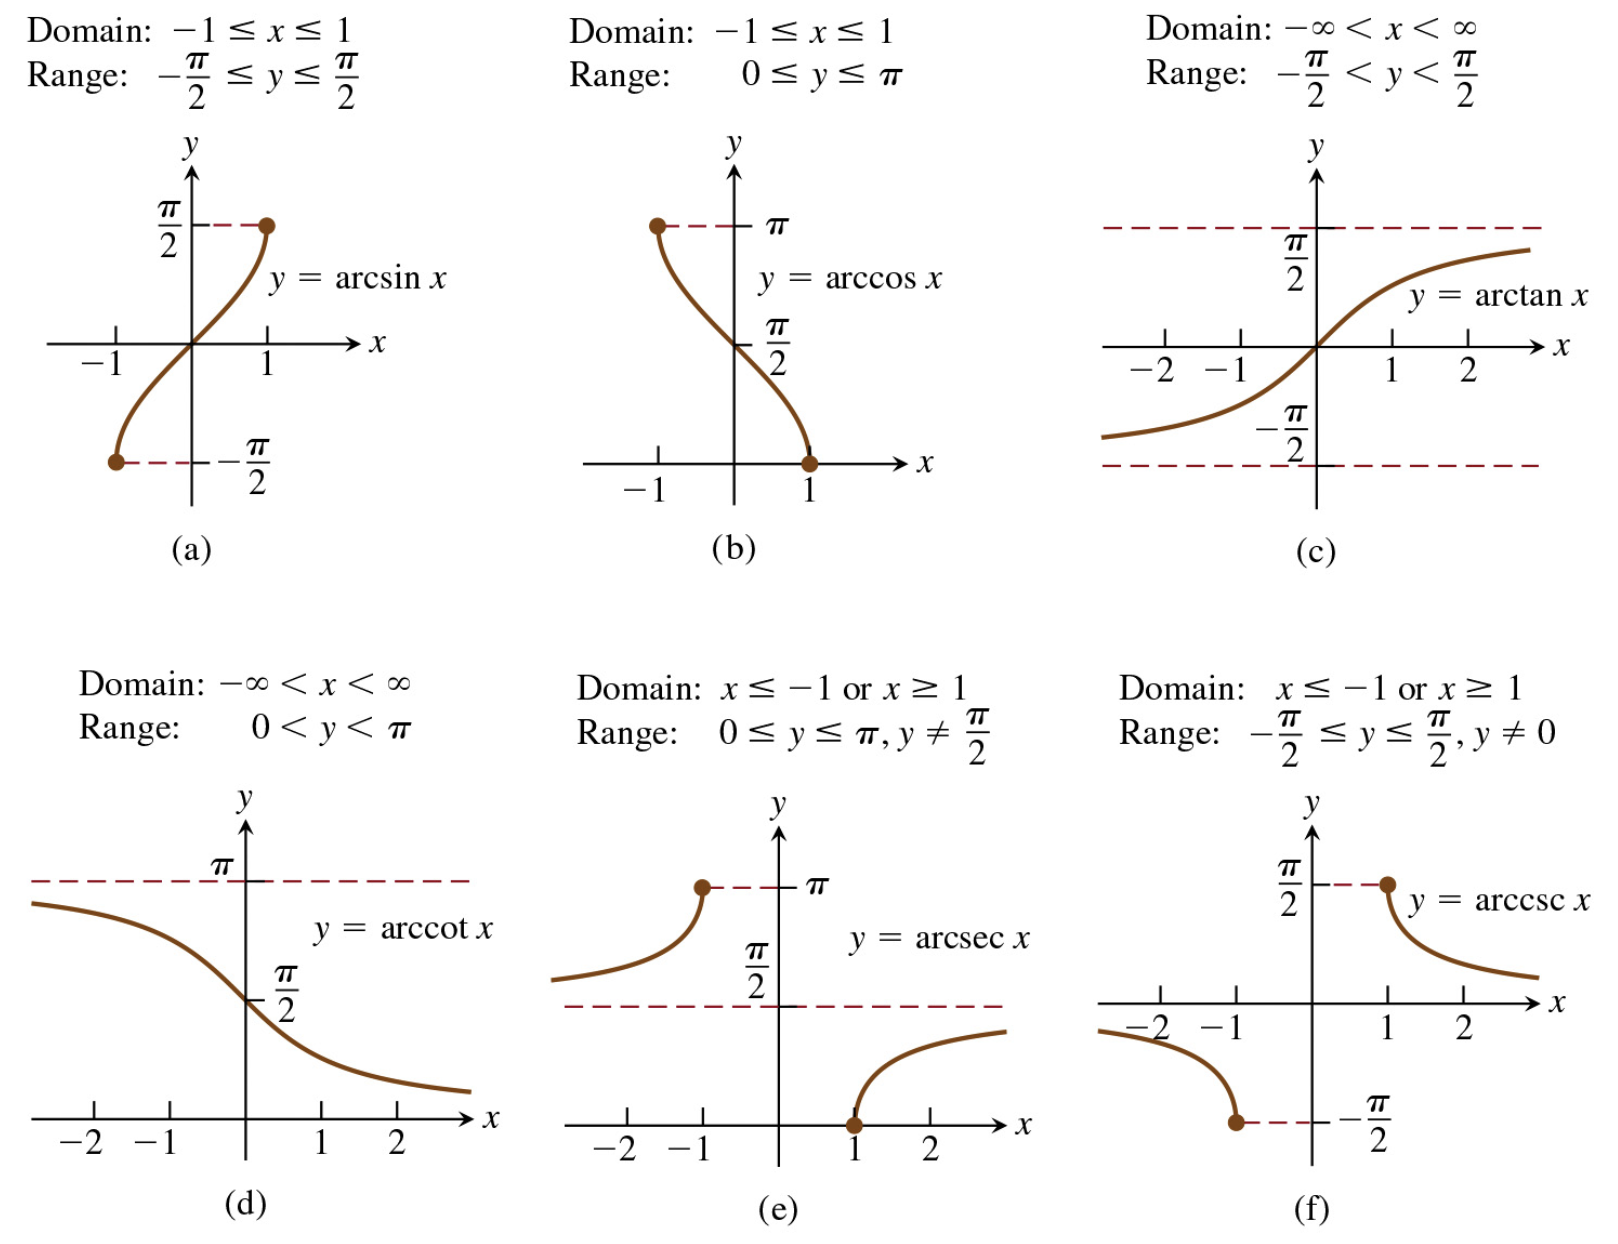
\includegraphics[width=6.5in]{img/inverse_trig_graphs}

\newpage

\begin{example}
Evaluate the following.
\begin{enumerate}
\item $\arcsin(\sqrt 3/2)$
\ifdefined\SOLUTION
\SOLUTION[Solution]{
\begin{equation*}
    \arcsin(\sqrt 3/2) = \theta \iff  \sin{\theta} = \frac{\sqrt{3}}{2} \text{ and } \theta \in [-\frac{\pi}{2}, \frac{\pi}{2}].
\end{equation*}
Because of the 30/60/90 (or $\frac{\pi}{6}$/$\frac{\pi}{3}$/$\frac{\pi}{2}$) triangle  with side lengths $1, \sqrt{3},$ and $2,$ it follows that $\sin{\frac{\pi}{3}} = \frac{\sqrt{3}}{2}.$  So, $\theta = \frac{\sqrt{3}}{2}.$  Therefore, $\arcsin(\sqrt 3/2) = \frac{\pi}{3}.$
}
\fi
\vfill

\item $\arcsin(-\sqrt 2/2)$
\ifdefined\SOLUTION
\SOLUTION[Solution]{
\begin{equation*}
    \arcsin(-\frac{\sqrt 2}{2}) = \theta \iff 
    -\frac{\sqrt 2}{2} = -\frac{1}{\sqrt{2}} =\sin{\theta}
    \text{ and } \theta \in \left[ -\frac{\pi}{2}, \frac{\pi}{2} \right].
\end{equation*}
Since $\sin{\theta} < 0,$ we need $\theta \in [0, -\frac{\pi}{2}),$ which is quadrant 4 of the unit circle.  Because of the triangle with angles $\frac{\pi}{4}, \frac{\pi}{4}, \frac{\pi}{2}$ and sides $1,1, \sqrt 2,$ it follows that $\sin{(-\frac{\pi}{4})} = -\frac{\sqrt 2}{2}.$  So, $\arcsin{(-\frac{\sqrt{2}}{2})} = -\frac{\pi}{4}.$
}
\fi
\vfill

\newpage

\item $\arccos(-1/2)$
\ifdefined\SOLUTION
\SOLUTION[Solution]{
\begin{equation*}
    \arccos(-1/2) = \theta \iff -1/2 = \cos{\theta} \text{ and } \theta \in [0,\pi].
\end{equation*}
Since $\cos{\theta} < 0,$ we need $\theta \in (\frac{\pi}{2}, \pi]$ (Quadrant 2).  The reference angle is $\alpha = \frac{\pi}{3}.$  So, $\theta = \pi - \frac{\pi}{3} = \frac{2\pi}{3}.$  Therefore, $\arccos{(-\frac{1}{2})} = \frac{2\pi}{3}.$
}
\fi
\vfill

\item $\arcsin(\sin(5\pi/8))$
\ifdefined\SOLUTION
\SOLUTION[Solution]{
\begin{equation*}
    \arcsin(\sin(5\pi/8)) = \theta 
    \iff \sin(5\pi/8) = \sin\theta \text{ and } \theta \in \left[ -\frac{\pi}{2}, \frac{\pi}{2} \right].
\end{equation*}
Since $\sin\theta > 0,$ $\theta$ is in Quadrant 1. Let $\alpha$ 
be the reference angle. So, 
\begin{equation*}
    \alpha = \theta = \pi - \frac{5\pi}{8} = \frac{3\pi}{8}.
\end{equation*}
Therefore, $\arcsin(\sin(5\pi/8)) = \frac{3\pi}{8}$.
}
\fi
\vfill
\end{enumerate}
\end{example}

\newpage

\begin{theorem}
\begin{align}
\frac{\dee}{\dee x}\arcsin x &= \frac{1}{\sqrt{1-x^2}}\quad (|x|<1),\label{derivative of arcsine}\\
\frac{\dee}{\dee x}\arccos x &= \frac{-1}{\sqrt{1-x^2}}\quad (|x|<1),\\
\frac{\dee}{\dee x}\arctan x &= \frac{1}{1+x^2},\\
\frac{\dee}{\dee x}\arccsc x &= \frac{-1}{|x|\sqrt{x^2-1}}\quad (|x|>1),\\
\frac{\dee}{\dee x}\arcsec x &= \frac{1}{|x|\sqrt{x^2-1}}\quad (|x|>1),\\
\frac{\dee}{\dee x}\arccot x &= \frac{-1}{1+x^2}.
\end{align}
\end{theorem}

\ifdefined\SOLUTION
\SOLUTION[Proof of~\eqref{derivative of arcsine}]{
By definition of arcsine, 
\begin{equation*}
    \sin(\arcsin(x)) = x \quad (-1\le x\le 1).
\end{equation*}
By the chain rule, 
\begin{equation*}
    \cos(\arcsin(x))\cdot\frac{\dee}{\dee x}\left(\arcsin x \right) = 1 \quad (-1<x<1),
\end{equation*}
and so, 
\begin{equation*}
\frac{\dee}{\dee x}(\arcsin x) = \frac{1}{\cos(\arcsin(x))} \quad (|x| < 1).
\end{equation*}
Note that for $|x|<1$, it follows that $\cos(\arcsin(x)) > 0$ and hence
\begin{equation*}
\cos(\arcsin(x)) = |\cos(\arcsin x)| = \sqrt{\cos^2(\arcsin x)} = \sqrt{1-\sin^2(\arcsin x)} = \sqrt{1-x^2}.
\end{equation*}
Thus, it follows that
\begin{equation*}
\frac{\dee}{\dee x}(\arcsin x) = \frac{1}{\sqrt{1-x^2}} \quad (|x| < 1).
\end{equation*}
}
\vfill
\else
\begin{proof}[Proof of~\eqref{derivative of arcsine}]\,

\vspace{3.5in}
\end{proof}
\fi

\begin{corollary}
\begin{align}
\int \frac{\dee x}{\sqrt{1-x^2}} &= \arcsin x + C\quad (|x|<1),\\
\int \frac{\dee x}{1+x^2} &= \arctan x + C,\\
\int \frac{\dee x}{x\sqrt{x^2-1}} &= \arcsec|x| + C\quad (|x|>1).
\end{align}
\end{corollary}

\newpage

\begin{example}
Compute $\dee y/\dee x$ if $y=\arcsin x^2$.
\end{example}
\ifdefined\SOLUTION
\SOLUTION[Solution]{
\begin{equation*}
    \frac{\dee y}{\dee x} = \frac{1}{\sqrt{1-(x^2)^2}}\cdot \frac{\dee}{\dee x}x^2 = \frac{2x}{\sqrt{1-(x^2)^2}}
\end{equation*}
}
\else
\fi
\vfill

\begin{example}
Evaluate the following.
\begin{enumerate}
\item $\DS\int_{\sqrt 2/2}^{\sqrt 3/2}\frac{\dee x}{\sqrt{1-x^2}}$
\ifdefined\SOLUTION
\SOLUTION[Solution]{
\begin{equation*}
    \int_{\sqrt 2/2}^{\sqrt 3/2}\frac{\dee x}{\sqrt{1-x^2}}
    = \arcsin(x)\Big|_{\sqrt 2/2}^{\sqrt 3/2}
    = \arcsin(\sqrt 3/2)-\arcsin(\sqrt 2/2)
    = \pi/3 - \pi/4
    = \frac{4\pi}{12}-\frac{3\pi}{12}
    = \frac{\pi}{12}
\end{equation*}
}
\fi
\vfill
\vfill

\item $\DS\int\frac{\dee x}{\sqrt{3-4x^2}}$
\ifdefined\SOLUTION
\SOLUTION[Solution]{
\begin{equation*}
    \int\frac{\dee x}{\sqrt{3-4x^2}} 
    = \frac{1}{\sqrt{3}}\int\frac{\dee x}{\sqrt{1 - \frac{4x^2}{3}}}
    = \frac{1}{\sqrt{3}}\int\frac{\dee x}{\sqrt{1 - (\frac{2x}{\sqrt 3}})^2}
\end{equation*}
Let $u = \frac{2x}{\sqrt{3}}.$  Then, $\dee u = \frac{2}{\sqrt{3}}\dee x.$  Making the substitution gives 
\begin{equation*}
    \frac{1}{2}\int\frac{\frac{2}{\sqrt 3}\dee x}{\sqrt{1 - (\frac{2x}{\sqrt 3}})^2}
    =  \frac{1}{2} \arcsin(\frac{2x}{\sqrt 3}) + C
\end{equation*}
}
\fi
\vfill
\vfill
\vfill
\end{enumerate}
\end{example}

\newpage

\begin{example}
Compute the following integrals.
\begin{enumerate}
\item $\DS\int\frac{\dee x}{\sqrt{\E^{2x}-6}}$
\ifdefined\SOLUTION
\SOLUTION[Solution]{
\begin{equation*}
    \int\frac{\dee x}{\sqrt{\E^{2x}-6}}
    = \frac{1}{\sqrt 6}\int\frac{\dee x}{\sqrt{\left(\frac{\E^x}{\sqrt{6}}\right)^2-1}}
\end{equation*}
Let $u = \frac{\E^x}{\sqrt 6}$ for $u > 0.$ So, $\dee u = \frac{\E^x}{\sqrt 6} \dee x = u \dee x.$ Dividing both sides by $u$ gives $\frac{\dee u}{u} = \dee x.$  Making the substitution gives 
\begin{equation*}
    \frac{1}{\sqrt 6}\int \frac{\frac{\dee u}{u}}{\sqrt{u^2-1}}
    =  \frac{1}{\sqrt 6}\int \frac{\dee u}{|u|\sqrt{u^2-1}}
    = \frac{1}{\sqrt 6}\arcsec(u) + C
    = \frac{1}{\sqrt 6}\arcsec(\frac{\E^x}{\sqrt{6}}) + C.
\end{equation*}
(The absolute value can be added around $u$ because $u > 0.$)
}
\else
\fi
\vfill

\item $\DS\int\frac{\dee x}{\sqrt{4x-x^2}}$
\ifdefined\SOLUTION
\SOLUTION[Solution]{
First, we rewrite $4x-x^2$ using algebra.
\begin{equation*}
    4x-x^2 = -(x^2-4x+4) + 4
    = -(x-2)^2 + 4
    = 4 - (x-2)^2
    = 4 \left[ 1-\left(\frac{x-2}{2}\right)^2 \right].
\end{equation*}
Rewriting the integral gives 
\begin{equation*}
    \int\frac{\dee x}{\sqrt{4x-x^2}}
    = \int\frac{\dee x}{2\sqrt{1-\left(\frac{x-2}{2}\right)^2}}
    = \arcsin{\left( \frac{x-2}{2} \right)} + C.
\end{equation*}
}
\fi
\vfill
\newpage

\item $\DS\int\frac{\dee x}{4x^2+4x+2}$
\ifdefined\SOLUTION
\SOLUTION[Solution]{
First, we rearrange the denominator of the fraction.  This can be done in two ways.  The first is 
\begin{equation*}
    4x^2 + 4x + 2 = 4(x^2 + x + 1/4) + 2 - 1
    = 4\left(x^2+1/2\right)^2 + 1
    = 2^2\left(x^2+1/2\right)^2 + 1
    =\left(2x^2+1\right)^2 + 1.
\end{equation*}
The second method is
\begin{equation*}
    4x^2 + 4x + 2 = (2x)^2 + 2(2x) + 2
    = \left[ (2x)^2 + 2(2x) + 1 \right] + 2 - 1
    = (2x + 1)^2 + 1.
\end{equation*}
So, the integral can be rewritten, giving
\begin{equation*}
    \int\frac{\dee x}{4x^2+4x+2}
    = \int\frac{\dee x}{(2x+1)^2 + 1}
    = \frac{1}{2} \int\frac{2\dee x}{(2x+1)^2 + 1}
    = \frac{1}{2}\arctan{(2x+1)} + C.
\end{equation*}
}
\else
\fi
\vfill
\end{enumerate}
\end{example}
